\chapter{Lecture 3}
\section{Entropy}
It is quite possible that the information source produces more than 1 letter at a time, i.e the source output is a sequence $u_1,u_2, \dots$ of letters. We can also consider the code $c_n: \Ucal^n \to \binset$.
\begin{eg}
We can take $\Ucal = \{a,b,c\}$ and have $c_2$ as $c(aa) = 0$, $c(ab)=10$, $c(ac) = 110$ etc.
\end{eg}
We can extend the notion from previous lecture for code $c_n$ as follows -- if $c_n: \Ucal^n \to \binset$ is uniquely decodable, then 
\[\EE[\ell(u_1 \dots u_n)] \geq \sum_{u_1, \dots, u_n} p(u_1, \dots, u_n) \log_2 \frac{1}{p(u_1, \dots, u_n)}\]
Moreover, there exists a prefix free code $\widetilde{c}_n$ also s.t.
\[\EE[\ell_{\widetilde{c}}(u_1 \dots u_n)] \leq \sum_{u_1, \dots, u_n} p(u_1, \dots, u_n) \log_2 \frac{1}{p(u_1, \dots, u_n)} + 1\]
A more interesting quantity to look at is the number of bits per letter. Hence, we have 
\[\frac1n\EE[\ell(u_1 \dots u_n)] \geq \frac{1}{n}\sum_{u_1, \dots, u_n} p(u_1, \dots, u_n) \log_2 \frac{1}{p(u_1, \dots, u_n)}\]
\[\frac1n\EE[\ell_{\widetilde{c}}(u_1 \dots u_n)] \leq \frac{1}{n}\sum_{u_1, \dots, u_n} p(u_1, \dots, u_n) \log_2 \frac{1}{p(u_1, \dots, u_n)} + \frac{1}{n}\]
Notice that as $n$ gets large, the two bounds are extremely close.
\begin{definition}
When $U \in \Ucal$ is a random variable, we define its entropy as 
\[
H(U) = \sum_u p(u) \log\frac{1}{p(u)}
\]
where $p(u) = \Pr[U=u]$.
\end{definition}
Thus, in terms of entropy, we can state that for any uniquely decodable code $c:\Ucal \to \binset$ and for any random variable $U \in \Ucal$,
\[\EE[\ell(U)] \geq H(U)\text{ and $\exists$ prefix free }\widetilde{c} \text{ s.t. } \EE[\ell_{\widetilde c}(U)] \leq H(U) + 1\]
Again, replacing $U$ $U_1, \dots U_n$, we get for any uniquely decodable $c_n: \Ucal^n \to \binset$ such that
\[\frac1n\EE[\ell(u_1 \dots u_n)] \geq \frac{1}{n}H(u_1, \dots, u_n)\]
Moreover there exists a prefix free code $\widetilde{c}_n$ s.t.
\[\frac1n\EE[\ell_{\widetilde{c}}(u_1 \dots u_n)] \leq \frac{1}{n}H(u_1, \dots, u_n) + \frac{1}{n}\]
\begin{eg}
Consider $\Ucal = \{a,b\}$ with $p(a) =p$ and $p(b) = 1-p$. 

\noindent
\begin{minipage}{0.6\textwidth}
The entropy for the above is given as
\[H(U) = p\log\frac{1}{p} + (1-p)\log\frac{1}{p}\]
The above quantity is defined as the binary entropy function $h_2(p)$. It has a maxima at $p=\frac{1}{2}$ and $h_2(0.5) = 1$.
\end{minipage}
\hspace{0.1\textwidth}
\begin{minipage}{0.3\textwidth}
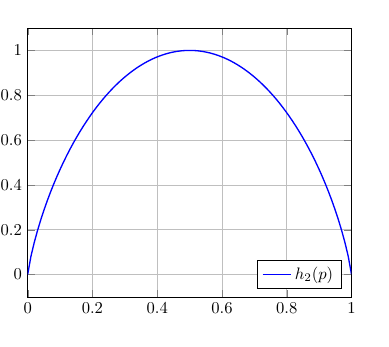
\begin{tikzpicture}[trim axis left, scale=0.6]
\begin{axis}[domain=0:1,
  samples=100,
  enlarge x limits=false,
  grid=both,
  no markers,
  legend pos=south east]
\addplot +[thick] {-x*log2(x) - (1-x)*log2(1-x)};
\addlegendentry{$h_2(p)$};
\end{axis}
\end{tikzpicture}
\end{minipage}
\end{eg}
\section{The Optimization Problem and Optimal Codes}
Consider the following - say we have an alphabet $\Ucal$ and a probability distribution $p$ defined on $\Ucal$ as input. At the output, we want the expected length of the codes to be minimum. Thus the output is $c:\Ucal\to\binset$ s.t. $c$ is prefix free and s.t. $\sum_u p(u) \ell(u)$ is as small as possible. We can frame this problem as
\[
\min \bigg\{ \sum_{u\in \Ucal} p(u) \ell(u) \; ;\; \sum_u 2^{-\ell(u)} \leq 1\bigg\} \text{ and } \ell(u) \in \NN
\]
The integer constraint makes the problem much tougher to solve. If that constraint is removed, the trivial solution is $\ell(u) = -\log p(u)$.
\begin{eg}
We can see another problem where integer constraint increases complexity. Consider the problem - given $w_1, \dots, w_k \geq 0$, and let $w = \sum w_i$. Find $S \subset \{1, \dots, k\}$ s.t. 
\[\min_S \bigg|\sum_{i\in S} w_i - \sum_{i\notin S}w_i\bigg| \equiv \min_S \bigg|\sum_{i\in S}w_i - \frac{w}{2}\bigg| \equiv \min_{x_1, \dots, x_k \in \{0,1\}} \bigg|\sum_{w_i x_i} - \frac{w}{2}\bigg|\]
If we remove the integer constraint, we can easily see that $x_i = \frac{1}{2}$ solves the problem.
\end{eg}
We have the following properties of optimal codes:
\begin{enumerate}
    \item If $p(u) < p(v)$ then $\ell(u) \geq \ell(v)$. The proof is trivial, because if that's not the case, we can swap $\ell(v)$ and $\ell(u)$ and improve the expected length of the code by $[p(v)-p(u)][\ell(v)-\ell(u)]$. 
    \begin{corollary}
    One of the longest codewords must belong to one of the least probable letters.
    \end{corollary}
    \item There have to be at least two longest codewords (assuming $|\Ucal| > 1$). Further, the two longest codewords must be siblings. This is also immediate - if there is a single longest codeword, it can be moved down the binary tree, and the codeword will get shorter.
    \begin{corollary}
    There is an optimal code in which the two least probable letters are assigned sibling codewords
    \end{corollary}
    \begin{proof}
    Consider a code $c$ in which the two least probable letters are not siblings. Just swap one of the codewords to make them siblings.
    \end{proof}
\end{enumerate}
In an optimal code for $(\Ucal, p)$, we know that the two least likely letters say $k$ and $k-1$ must have codewords $[\dots]0$ and $[\dots]1$. Let the common prefix $[\dots]$ have length $\widetilde{\ell}$. Then we can write
\begin{align*}
\EE[\ell(U)] &= p(1)\ell(1) + p(2)\ell(2) + \cdots + p(k-2)\ell(k-2) + [p(k) + p(k-1)](1+\widetilde{\ell}) \\
&= p(1)\ell(1) + \cdots + [p(k) + p(k-1)]\widetilde{\ell} + [p(k) + p(k-1)] \\
\end{align*}
Thus our optimization problem is as follows - 
\begin{align*}
&\min_{\ell(1), \dots, \ell(k)} \sum_{i=1}^k p(i)\ell(i) \text{ s.t. } \sum_i 2^{-\ell(i)} \leq 1 \\
\equiv &\min_{\ell(1),\cdots,\ell(k-2),\widetilde{\ell}}\sum_{i=1}^{k-2} p(i)\ell(i) + [p(k-1) + p(k)]\widetilde{\ell} + [p(k) + p(k-1)] \text{ s.t. } \Big(\sum_{i=1}^{k-2} 2^{-\ell(i)}\Big)+ + 2^{-\widetilde{\ell} - 1} + 2^{-\widetilde{\ell} - 1} \leq 1
\end{align*}
The constraint is same as $2^{-\ell(1)} + 2^{-\ell(2)} + \dots + 2^{-\ell(k-2)} + 2^{-\widetilde{\ell}} \leq 1$. Thus, we reduced the optimization problem to $k-1$ variables, i.e. $(\Ucal=\{1,\dots,k\}, p=(p(1),\dots,p(k)) \to (\Vcal=\{1,\dots,k-1\}, q=(p(1),\cdots,p(k-2),p(k-1)+p(k))$. We can keep on repeating this procedure and bring the problem down even from the $(\Vcal, q)$ code. 
\begin{eg}
We show the Huffman procedure on the following code: $\Ucal = \{a,b,\dots,f\}$ and $p = (0.25, 0.2, 0.15, 0.15, 0.15, 0.1)$.

\begin{tikzpicture}
[every node/.style={minimum height=2em}]
\matrix [matrix of math nodes](Mat)
{
x_i  &|[minimum width=2em]|& P(x_i) &|[minimum width=4em]| Code &       &|[minimum width=4em]|      &       &|[minimum width=4em]|  &   &|[minimum width=4em]|  &   &|[minimum width=4em]| &  &\\
a &&0.25     &        & 0.25  &   &0.25   &   &0.25&  &{\color{magenta}0.55}& & {\color{magenta}1}\\
b && 0.2    &        & 0.2  &   &0.2   &   &0.30&  &0.45& &\\
c && 0.15   &     & 0.15  &   &{\color{magenta}0.3}   &   &{\color{magenta} 0.45}&  &   & &\\
d && 0.15    &        &0.15   &   &0.25   &   &   &   &   & &\\
e && 0.15    &        &{\color{magenta}0.25}   &   &       &   &   &   &   & &\\
f && 0.1    &        &   &   &       &   &   &   &   & &\\
};

%\draw (Mat-2-3.east) -- (Mat-2-3-|Mat-2-5.west)node[above,midway]{00};
%\draw(Mat-5-3.east) --++(1em,0) -- (Mat-6-5.west)node[above,pos=0.2]{101};
\draw (Mat-6-3.east)-|node[above,pos=0.4]{\color{ForestGreen}110}++(2em,-1em) coordinate(aa) --++(1em,0) |- (Mat-6-5.west);
\draw (Mat-7-3.east)-|node[below,pos=0.4]{\color{ForestGreen}111} (aa);
\draw (Mat-4-5.east)-|node[above,pos=0.4]{\color{ForestGreen}010}++(2em,-1em) coordinate(aa) --++(1em,0) |- (Mat-4-7.west);
\draw (Mat-5-5.east)-|node[below,pos=0.4]{\color{ForestGreen}011} (aa);
\draw (Mat-3-7.east)-|node[above,pos=0.4]{\color{ForestGreen}10}++(2em,-1em) coordinate(aa) --++(1em,0) |- (Mat-4-9.west);
\draw (Mat-5-7.east)-|node[below,pos=0.4]{11} (aa);
\draw (Mat-2-9.east)-|node[above,pos=0.4]{\color{ForestGreen} 00}++(2em,-1em) coordinate(aa) --++(1em,0) |- (Mat-2-11.west);
\draw (Mat-3-9.east)-|node[below,pos=0.4]{01} (aa);
\draw (Mat-2-11.east)-|node[above,pos=0.4]{0}++(2em,-1em) coordinate(aa) --++(1em,0) |- (Mat-2-13.west);
\draw (Mat-3-11.east)-|node[below,pos=0.4]{1} (aa);
\end{tikzpicture}

Following the procedure, we get the codes (marked in green for the corresponding letter in the alphabet). The nodes marked in magenta are the fake nodes, and can be used to calculate the expected length of the code. 
The expected length of the code is given by
\[
\EE[\ell(u)] = \sum \text{(fake node values)} = 0.25 + 0.3 + 0.45 + 0.55 + 1 = 2.55
\]

\end{eg}